
% ----------------------------------------------------------------
% AMS-LaTeX Paper ************************************************
% **** -----------------------------------------------------------
\documentclass[11pt]{amsart}
\usepackage{graphicx, mathabx, amssymb,amsfonts,amsmath,amsthm,newlfont,mathtools}
\usepackage{epsfig,url}
\usepackage[usenames,dvipsnames]{color}
\usepackage{enumerate}
\usepackage[colorlinks=true,linkcolor=red,citecolor=blue]{hyperref}
\usepackage{color}
\usepackage{stmaryrd}         % Crochet double barre (entiers)

% !TEX root = ../Poissons.tex




%Clever ref
\usepackage[noabbrev,capitalize]{cleveref}
\usepackage[all,2cell]{xy} \UseAllTwocells \SilentMatrices

%MARGINS

\setlength{\textwidth}{\paperwidth}
\addtolength{\textwidth}{-2.5in}
\calclayout


% ----------------------------------------------------------------
\vfuzz2pt % Don't report over-full v-boxes if over-edge is small
\hfuzz2pt % Don't report over-full h-boxes if over-edge is small
% THEOREMS -------------------------------------------------------
\newtheorem{thm}{Theorem}[section]
\newtheorem{corollary}[thm]{Corollary}
\newtheorem{lemma}[thm]{Lemma}
\newtheorem{construction}[thm]{Construction}
\newtheorem{proposition}[thm]{Proposition}
\newtheorem{Questions}[thm]{Questions}
\theoremstyle{definition}
\newtheorem{definition}[thm]{Definition}

\newtheorem{conjectue}{Conjecture} 
\newtheorem{QQ}{Question} 
\newtheorem{prob}{Problem}
\newtheorem{ex}[thm]{Examples}
\newtheorem{example}[thm]{Example}
\newtheorem{policy}{Policy}
\theoremstyle{remark}
\newtheorem{rem}[thm]{Remark}
\newtheorem{caveat}[thm]{Caveat}
\numberwithin{equation}{section}
% MATH -----------------------------------------------------------
\newcommand{\norm}[1]{\left\Vert#1\right\Vert}
\newcommand{\abs}[1]{\left\vert#1\right\vert}
\newcommand{\set}[1]{\left\{#1\right\}}

\newcommand{\To}{\longrightarrow}
\newcommand*{\Longhookrightarrow}{\ensuremath{\lhook\joinrel\relbar\joinrel\rightarrow}}
\newcommand{\Z}{\mathbb Z}
\newcommand{\Q}{\mathbb Q}
\newcommand{\C}{\mathbb C}
\newcommand{\Ok}{\mathcal O}
\newcommand{\ai}{\mathfrak{a}}
\newcommand{\bi}{\mathfrak{b}}
\newcommand{\R}{\mathbb R}
\newcommand{\N}{\mathbb N}
\newcommand{\AM}{A}
\newcommand{\xx}{\mathsf{x}}
\newcommand{\eqv}{\mathrm{ev}}
\font \rus= wncyr10
\newcommand{\sha}{\, \hbox{\rus x} \,}

\newcommand{\Lie}{\mathrm{Lie}}

\newcommand{\GC}{\mathcal{GC}}
\newcommand{\q}{/\!/}

\newcommand{\tr}{\mathrm{tr}}
\newcommand{\id}{\mathrm{id}}

\newcommand{\can}{\mathrm{can}}

\newcommand{\mm}{\mathfrak{m}}

\newcommand{\GL}{\mathrm{GL}}
\newcommand{\LP}{L}
\newcommand{\FL}{F\!L}
\newcommand{\mc}{\mu}

%Important sets 
\newcommand{\EC}{\mathcal{E}} %essential complimentary partitions
\newcommand{\OP}{\triangle} %ordered partitions
\newcommand{\BT}{\mathcal{B}} %bipartite trees


\newcommand{\0}{\color{blue}{\mathsf{0}}}

%OEIS
\newcommand{\OEIS}[1]{{\rm \href{http://oeis.org/#1}{\texttt{#1}}}}

%Commentaires 

\newcommand{\Guillaume}[1]{\textcolor{magenta}{\underline{Guillaume}: #1}}
\newcommand{\Kurt}[1]{\textcolor{blue}{\underline{Kurt}: #1}}

\DeclareMathOperator{\Ima}{Im} %Image d'une fonction

%Drapeau européen

\usepackage{graphicx,calc}
\newlength\myheight
\newlength\mydepth
\settototalheight\myheight{Xygp}
\settodepth\mydepth{Xygp}
\setlength\fboxsep{0pt}
\newcommand*\inlinegraphics[1]{%
  \settototalheight\myheight{Xygp}%
  \settodepth\mydepth{Xygp}%
  \raisebox{-\mydepth}{\includegraphics[height=\myheight]{#1}}%
}

%Dessins

\usepackage{tikz}
\usepackage{tikz-cd}
\usepackage{pgfplots}
\usepackage{pgfplotstable}
\tikzset{math3d/.style=
    {x= {(-0.353cm,-0.353cm)}, z={(0cm,1cm)},y={(1cm,0cm)}}}
\tikzset{JLL3d/.style=
    {x= {(0.4cm,-0.2cm)}, z={(0cm,1cm)},y={(-1cm,0cm)}}}
\usetikzlibrary{calc}
\usetikzlibrary{shapes,shapes.geometric,fit,positioning,calc,matrix}
\tikzset{
  optree/.style={scale=.5,thick,grow'=up,level distance=10mm,inner sep=1pt},
  comp/.style={draw=none,circle,fill,line width=0,inner sep=0pt},
  dot/.style={draw,circle,fill,inner sep=0pt,minimum width=3pt},
  circ/.style={draw,circle,inner sep=1pt,minimum width=4mm},
  emptycirc/.style={draw,circle,inner sep=1pt,minimum width=2mm},
  root/.style={level distance=10mm,inner sep=1pt},
  leaf/.style={draw=none,circle,fill,line width=0,inner sep=0pt},
  nodot/.style={draw,circle,inner sep=1pt},
}

\pgfplotsset{compat=1.12}

% ----------------------------------------------------------------

\def\abovespace{\vspace{12pt}}
\def\belowspace{\vspace{8pt}}



\addtolength{\hoffset}{-0.0in} \addtolength{\textwidth}{0in}
\addtolength{\voffset}{-0.0in} \addtolength{\textheight}{0.0in}



% -----------------------------------------------------------------

\title{The combinatorics of the permutahedron diagonals}

\author[B. Delcroix-Oger]{B\'er\'enice Delcroix-Oger}
\address{Institut Montpelliérain Alexander Grothendieck, Université de Montpellier, France}
\email{berenice.delcroix-oger@umontpellier.fr}

\author[M. Josuat-Verg\`es]{Matthieu Josuat-Verg\`es}
\address{}
\email{}

\author[G. Laplante-Anfossi]{Guillaume Laplante-Anfossi}
\address{School of Mathematics and Statistics, University of Melbourne, Victoria, Australia}
\email{guillaume.laplanteanfossi@unimelb.edu.au}

\author[K. Stoeckl]{Kurt Stoeckl}
\address{}
\email{}

\date{\today}

\subjclass[2010]{Primary [...]; Secondary 18M70} 

\keywords{Polytopes [...]}


%\thanks{G. L.-A. was supported by }

%========================================
\begin{document}
%========================================

\begin{abstract}
The purpose of this note is to provide a new combinatorial description of a cellular approximation of the diagonal of the permutahedra. 
\end{abstract}


\maketitle


\setcounter{tocdepth}{1}
%\tableofcontents

% !TEX root = ../Poissons.tex

\section*{Introduction} 
\label{s:introduction}

The purpose of this article is to study cellular diagonals on the permutahedra, which are cellular maps homotopic to the usual thin diagonal $\triangle : P \to P \times P, x \mapsto (x,x)$.
Such diagonals, and in particular coherent families that we call \emph{operadic} diagonals (see [DEF]), are of interest in algebraic geometry and topology: via the theory of Fulton--Sturmfels \cite{fultonIntersectionTheoryToric1997a}, they give explicit formulas for the cup product on Losev--Manin toric varieties \cite{losevNewModuliSpaces2000}; they define universal tensor products of homotopy operads, and in particular universal tensor products of homotopy associative permutads (shuffle algebras) \cite{LA21}; they allow for the definition of a coproduct on permutahedral sets, which are used to models of two-fold loop spaces \cite{SaneblidzeUmble04}; and their study is moreover needed to pursue the work of Baues aiming at defining explicit combinatorial models for higher iterated loop spaces \cite{bauesGeometryLoopSpaces1980}. 
Moreover, using the canonical projections to the multiplihedra and the associahedra, they define universal tensor product of $\Ainf$-algebras and $\Ainf$-morphisms \cite{MazuirLA22}.
\Guillaume{lien avec les matroides?}

The first cellular diagonal for the permutahedra was defined at the level of chains by S. Saneblidze and R. Umble in \cite{SaneblidzeUmble04}, we will call it the \emph{SU diagonal}. 
Cellular diagonals for the associahedra and the multiplihedra were also defined there, via projection. 
The first topological map for the permutahedra was given in \cite{LA21} -we will call it the \emph{LA diagonal}, where a general theory of cellular diagonals of polytopes was developed. 
The LA diagonal, however, is distinct from the SU diagonal at the cellular level \cite[Remark 3.19]{LA21}. 

computer program for the SU diagonal \cite{vejdemo-johanssonEnumeratingSaneblidzeUmbleDiagonal2007}; we give a much more effective computer program (however, without the signs)

corollary: le dernier article de SU!
corollary: IJ-description of SU diagonal
corollary: left and right shifts for LA, decomposition of the cube associated to LA diagonal



\subsection{Conventions}
%We use the notations of \cite{LodayVallette12} for operads.

\Guillaume{Please make a new line for each sentence as to facilitate comparison between versions in GitHub}

\Guillaume{Would it be possible to avoid bold letters, use "slash emph\{\}", and also reduce to the maximum possible the use of indices; as soon as the context is clear, drop any extra index}




% !TEX root = ../Poissons.tex

\section{Higher Algebra}

\subsection{Operadic diagonals}

\subsubsection{Cellular diagonals}

The usual \emph{thin diagonal} of a topological space $X$ is the map $\Delta : X \to X \times X$ defined by $\Delta(x):=(x,x)$ for all $x \in X$.

\begin{definition}
    A \emph{cellular diagonal} of a polytope $P$ is a continuous map $P \to P \times P$ such that
    \begin{enumerate}
        \item its image is a union of $\dim P$-faces of $P\times P$ (i.e. it is \emph{cellular}),
        \item it agrees with the thin diagonal on the vertices of $P$, and
        \item it is homotopic to the thin diagonal, relative to the image of the vertices. 
    \end{enumerate}
    A cellular diagonal is said to be \emph{face-coherent} if its restriction to a face of $P$ is itself a cellular diagonal for that face. 
\end{definition}

A powerful geometric technique to define face-coherent cellular diagonals on polytopes first appeared in \cite{fultonIntersectionTheoryToric1997a}, was presented in \cite{masudaDiagonalAssociahedra2021}, and was fully developed in \cite{LA21}.
The key idea is the following: any vector $\vec v$ in generic position with respect to $P$ defines a cellular diagonal $\triangle_{(P,\vec v)}$, via the following formula
\begin{align*}
    \begin{array}{rlcl}
    \triangle_{(P,\vec v)}\  : & P &\to  &P\times P\\
    &z & \mapsto& 
    \bigl(\min_{\vec v}(P\cap \rho_z P),\,  \max_{\vec v}(P\cap \rho_z P)\bigr) \ .
    \end{array}
\end{align*}
Here, $\rho_z P := 2z-P$ denotes the reflection of $P$ with respect to the point $z$, and $\min_{\vec v}(P)$ denotes the unique vertex of $P$ which minimizes the scalar product with $\vec v$. 
The diagonal $\triangle_{(P,\vec v)}$ defines a canonical polytopal subdivision of $P$: it is by construction a tight coherent section of the projection $\pi : P \times P \to (P+P)/2$, and one just needs to draw the polytopes $(F+G)/2$, for all pairs of faces $(F,G) \in \Ima \triangle_{(P,\vec v)}$.

\begin{definition}
    The \emph{$f$-vector} of the diagonal $\triangle_{(P,\vec v)}$ is the number of faces of $P\times P$ of given total dimension in its cellular image.
    Alternatively, it is the $f$-vector of the polytopal complex~$\pi (\triangle_{(P,\vec v)})$.
\end{definition}

For the purpose of studying this $f$-vector, one can study the dual of the polytopal complex.

\begin{proposition}
    The $f$-vector of a cellular diagonal of the permutahedron $\triangle_{(P,\vec v)}$ is given by the opposite of the $f$-vector of the hyperplane arrangement made of the braid arrangement together with a second copy of it, translated in the generic direction $\vec v$. 
\end{proposition}

\begin{proof}
    This follows from \cite[Proposition 1.3]{LA21}; \cite[Corollary 1.4]{LA21} describes precisely the intersection poset of this hyperplane arrangement.
\end{proof}
 
The first part of the paper provides explicit formulas for this $f$-vector. 

\subsubsection{The $\LA$ diagonal on the permutahedra}

Let us first set up some notations that will be of use throughout the paper. 
A set $\sigma_I := \bigcup_{i\in I} \sigma_i$ is a \emph{partition} of $[n]:=\{1,\ldots,n\}$ if $\bigcup_{i\in I} \sigma_i = [n]$ and $\sigma_i \cap \sigma_j = \emptyset$ for $i \neq j$.
The subsets $\sigma_i$ are called \emph{blocks}. 
We denote by $|\sigma|:=|I|$ the size of the partition (its number of blocks).
A partition is \emph{ordered} if the indexing set $I$ is equipped with a total order; in what follows we shall use $I=[k]$ for $k \in \N$. 
We use the shorthand $14|23$ to denote both the unordered  partition $\{\{1,4\},\{2,3\}\}$, and also the ordered partition $(\{1,4\},\{2,3\})$ (when the order is clear from context).

Let us recall the combinatorial formula for the cellular approximation of the diagonal of the permutahedra from \cite[Theorem 3.16]{LA21}.
Let $n\geq 1$, and let us write \[ \LA(n) \coloneqq \{(I,J) \ | \ I,J\subset\{1,\ldots,n\}, |I|=|J|, I\cap J=\emptyset, \min(I\cup J)\in I \}. \] 
Let $\vec v \in \R^n$ be such that $\forall (I,J) \in \LA(n)$, we have $\sum_{i \in I} v_i > \sum_{j \in J} v_j$, and let $P\subset \R^n$ denote the standard $(n-1)$-dimensional permutahedron.
For any pair $(\sigma,\tau)$ of ordered partitions of $[n]$, we have
\begin{eqnarray*}
    (\sigma,\tau)\in \Ima\triangle_{(P,\vec v)} 
    & \iff & \forall (I,J) \in D(n), \exists k \in [n] , 
    \left| \sigma_{[k]} \cap I \right|
    >
    \left| \sigma_{[k]} \cap J \right| \text{ or } \\
    && \exists l \in [n] , 
    \left| \tau_{[l]} \cap I \right|
    <
    \left| \tau_{[l]} \cap J \right|  \ . 
\end{eqnarray*}
We shall denote by $\LAD$ the set of pairs of ordered partitions of $[n]$ which satisfy the above condition. 
There is an equivalent description of $\LAD$ which has the following form: 
\begin{proposition}
\label{p:minimal}
For a two ordered partitions $\sigma, \tau \subset [n]$, we have
\begin{eqnarray*}
    (\sigma,\tau)\in \LAD 
    & \iff & \forall (I,J) \in \LA(\sigma,\tau), \exists k \in [n] , 
    \left| \sigma_{[k]} \cap I \right|
    >
    \left| \sigma_{[k]} \cap J \right| \text{ or } \\
    && \exists l \in [n] , 
    \left| \tau_{[l]} \cap I \right|
    <
    \left| \tau_{[l]} \cap J \right|  \ . 
\end{eqnarray*}
\end{proposition}
Here, $\LA(\sigma,\tau) \subset \LA(n)$ is a proper subset of $\LA(n)$ which depends on the choice of~$(\sigma,\tau)$, and comes from the geometry of the situation, see \cite[Theorem 1.26]{LA21} for more details.
For our present purposes, it will be enough to restrict our attention to facets of $\LA$, that is pairs $(\sigma,\tau)$ which satisfy $|\sigma| + |\tau|=n+1$.
In this case, $\LA(\sigma,\tau)$ has $n-1$ elements, and admits the following description. 

For any subset $\sigma_i \subset [n]$, let $\vec \sigma_i \in \R^n$ denote the boolean vector whose coordinates are given by $1$ in position $j$ if $j \in \sigma_i$ and $0$ otherwise. 
Given a facet $(\sigma,\tau)$ of $\LAD$, one can consider the system of equations $\langle \vec \sigma_i , x \rangle=0$, $\langle \vec \tau_j , x \rangle=0$ given by the blocks of both partitions.
For geometric reasons (see the proof of \cite[Theorem 1.26]{LA21}), the solution of this system is $x=0$. 
Now we will be interested in the solutions of the systems associated to the pairs $(\sigma',\tau)$ and $(\sigma,\tau')$ where $\sigma'$ (resp. $\tau'$) has been obtained from $\sigma$ (resp. $\tau$) by merging two adjacent blocks.

\begin{proposition}
\label{p:minimal-IJ-pairs}
    There is a bijection between the set $\LA(\sigma,\tau)$ and the solutions to the systems of equations of the form $(\sigma',\tau)$ and $(\sigma,\tau')$. 
\end{proposition}

\begin{proof}
    For any $z \in (\mathring \sigma+ \mathring \tau)/2$, the face $\tau \cap \rho_z \sigma$ of $P \cap \rho_z P$ is a vertex of the polytope $P \cap \rho_z P$.
    The faces of the form $\tau \cap \rho_z \sigma'$ and $\tau' \cap \rho_z \sigma$ are the edges of $P\cap \rho_z P$ which are adjacent to the vertex $\tau \cap \rho_z \sigma$. 
    By definition $D(\sigma, \tau)$ describes the directions of these edges, and the translation is made as follows: for a given pair $(I,J)$, define the corresponding direction $\vec d$ by its coordinates $d_i:=1$ if $i \in I$, $d_j:=-1$ if $j \in J$, and $d_k:=0$ otherwise.  
    We refer to \cite[Section 1.5]{LA21} for more details.
\end{proof}

We will sometimes refer to the elements of $\LA(\sigma,\tau)$ as the \emph{minimal $(I,J)$-pairs}.




% !TEX root = ../Poissons.tex

\section{Facets of the diagonal} 
\label{s:facets}

In this section we establish a bijection between the facets of $\triangle$ and a family of pairs of unordered partitions introduced and enumerated in a series of 3 papers \cite{chen1969computer,chen1971tables,kajitani1982number}. An intermediary bijection to a type of bipartite tree is of particular importance and provides [...].
In particular, we obtain that the number of facets in $\triangle_n$ is $2(n+1)^{n-2}$ (\OEIS{A007334}), and more precisely that the pairs of dimension $(k,n-k)$ are counted by the formula $\binom{n}{k+1}(k+1)^{n-k-1}(n-k)^{k-1}$.

\Guillaume{Notations to be uniformized...}

\subsection{Essential complementary partitions and bipartite trees}
Let us recall some basic definitions and results from the series of papers \cite{chen1969computer,chen1971tables,kajitani1982number}.

\begin{definition}
A set of \emph{distinct representatives} of a partition is a set $R\subset [n]$ such that $\forall i \in I,|P_i \cap R| = 1$.
\end{definition}

\begin{definition}
A pair of partitions $P=(P_L,P_R):=(\cup_{l\in L} P_l , \cup_{r\in R} P_r)$ is
\begin{itemize}
    \item \emph{complimentary} if there exists $I\subset [n]$ and $p \in I$ such that $I$ and $(V\setminus I) \cup \{p\}$ are distinct representatives of $P_L$ and $P_R$, respectively.
    \item \emph{essential} if there does not exists proper subsets $K \subset [n], L'\subset L$ and $R'\subset R$ such that $P':=(P_{L'},P_{R'})$ is a complimentary partition of $K$.
\end{itemize}
\end{definition}

We shall denote the set of all essential complimentary pairs of partitions by $\EC$.
Let us emphasize that the pairs of partitions of $\EC$ are \emph{unordered}.

\begin{example}
n=2, n=3
\end{example}
\Kurt{To do}

A \emph{tree} is a simply connected graph with no cycles. 
A \emph{bipartite graph} is a graph whose vertices are partitioned into two sets such that vertices in one set are only adjacent to vertices in the other, we say it is \emph{ordered} if one of the sets is considered smaller than the other and we denote the partition $(V_L,V_R)$. 
We say a graph with $n$ edges is \emph{edge labelled} if there exists a bijection between the edges and $\{1,\dots,n\}$.
Let $\BT$ denote the set of edge labelled ordered bipartite trees.

\begin{proposition} [{\cite[Theorem 3]{kajitani1982number}}] 
\label{EC Graph Bijection}
Essential complementary partitions and labelled bipartite trees are in bijection through $G:\EC \to \BT$ and $P:\BT \to \EC$, where
\begin{itemize}
    \item $G$ takes a pair $(P_L,P_R)$ and constructs partitioned vertices $(V_L,V_R)$. For each $i \in  \{1,\dots,n\}$ an edge is added between $v_l$ and $v_r$ if $i\in P_l$ and $i \in P_r$. 
    \item $P$ takes a tree from $\BT$ and labels the vertices $(V_L,V_R)$ by the edges which are adjacent to them. The labels of the vertices can then be interpreted as a pair of partitions.
\end{itemize}
\end{proposition}
\Guillaume{Consider changing notation for functions vs sets}

\begin{figure}
\begin{center}
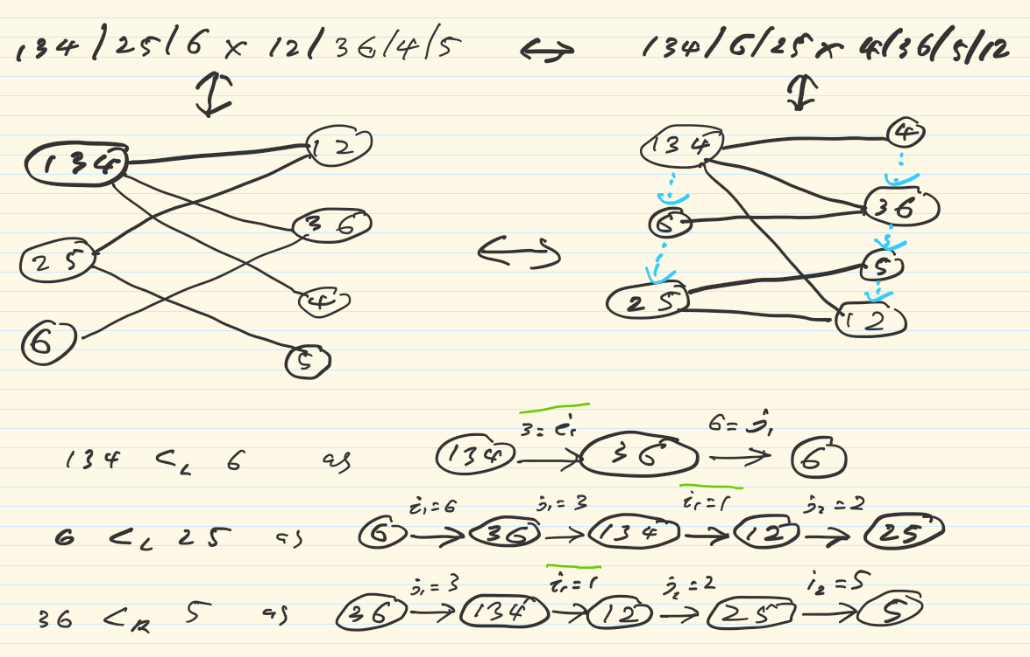
\includegraphics{Images/bijections_example.png}
\end{center}
\caption{The bijection between ordered partitions and bipartite trees.}
\end{figure}

\begin{corollary}[\cite{kajitani1982number}]
The number of essential complementary partitions is $|\EC_n| = 2(n+1)^{n-2}$.
\end{corollary}

\subsection{Bijection with the facets of the diagonal}

In this section we denote by $\OP$ be the set of pairs of ordered partitions of $[n]$ labeling \emph{facets} of the diagonal $\triangle$.

\begin{thm}
\label{thm:facets}
Facets of the diagonal and essential complimentary partitions are in bijection through the inverse functions $u:\OP \to \EC$ and $o:\EC\to \OP$, where
\begin{enumerate}
    \item The function $u$ forgets the order of the ordered partition pair.
    \item The function $o$ uniquely orders an essential complimentary partition pair via the minimal $(I,J)$-pairs defining the diagonal. 
\end{enumerate}
\end{thm}
We shall prove this theorem by establishing the necessary total order, showing that the functions are well defined, and then showing that they are injective.

\begin{lemma} 
\label{u well defined}
The function $u:\OP \to \EC$ that forgets the order in a pair of partitions is well defined.
\end{lemma}
\begin{proof}
Let $P \in \OP_n$. Then $G(u(P))$ is a graph with $l+r=n+1$ vertices, and $n$ edges. Furthermore, as no vertices can be isolated it must be the case that this graph is a tree. 
It is straightforward to verify that $G(u(P))$ must be labeled bipartite tree, but here is how we may explicitly produce the necessary distinct representatives using an algorithm of \cite[Theorem 2]{kajitani1982number}.

Let $G'$ be a copy of $G(u(P))$. 
While there is a vertex of degree $1$ in $G'$ delete it and add the sole edge of that vertex as a distinct representative of the corresponding partition of that vertex. 
As $G'$ is a tree this process can continue until there is a single edge connecting two vertices of degree $1$. 
This edge specifies the element $p$ of the distinct representatives.
\end{proof}

\begin{construction} 
\label{Order Lemma}
For $P=(P_L,P_R) \in \EC$ an essential complementary pair, we construct total orders on $P_L$ and $P_R$ in three steps:
\begin{enumerate}
    \item For $l,l' \in L$ there exists a unique minimal set of edges $p_{l,l'}$ of even cardinality connecting $V(P_l)$ and $V(P_{l'})$ in $G(P)$ (similar for $R$). We partition this set of edges as $I\cup J$ where $I$ and $J$ are each pairwise non-adjacent, and $I$ contains the minimal edge.
    \item Orient each path so that $I$ points left to right, and $J$ points right to left (same orientation for $P_L$ and $P_R$). 
    \item We say $P_l< P_{l'}$ (or $P_r < P_{r'}$) if the constructed path points from $V(P_l) \to V(P_{l'})$ ($V(P_r) \to V(P_{r'})$.
\end{enumerate}
\end{construction}

\begin{proof}
We first show our binary relation is well defined before verifying that it defines a total order on $G(P)$ and hence $P$ via the bijection of \cref{EC Graph Bijection}.

As $G(P)$ is a bipartite tree, every vertex is connected, and every path connecting two vertices on the same side must be of even length. 
As $I$ and $J$ are each pairwise non-adjacent, they must partition the path in an alternating fashion i.e. $p=(I_{i_1},J_{j_1},I_{i_2},J_{j_2},..., )$, hence we can orient the path by forcing $I$ to point left and $J$ to point right.

This order is clearly total, reflexive (by convention) and anti-symmetric, what remains to be checked is its transitivity. 

Let $p_{ab}$ denote the unique maximal path between two vertices $a$ and $b$ on the left of $G(P)$, that is two blocks of $P_L$. 
Let $I_{ab}$ denote the set of left-to-right edges in this path, and let $J_{ab}$ denote its complement. 
Then, we have 
\begin{equation}
    \label{eq:order}
    a < b \iff \min(I_{ab}\cup J_{ab})=\min(I_{ab}) \ . 
\end{equation}
Suppose now that $a < b$ and $b < c$.
Since $p_{ac}= (p_{ab} \cup p_{bc}) \setminus (p_{ab} \cap p_{bc})$, we have $$ I_{ac}=(I_{ab}\cup I_{bc}) \setminus (J_{ab} \cup J_{bc}) \text{ and } J_{ac}=(J_{ab}\cup J_{bc}) \setminus (I_{ab} \cup I_{bc}) \ , $$ and from the condition (\ref{eq:order}) above it is clear that $\min(I_{ac}\cup J_{ac})=\min(I_{ac})$, which completes the proof of the transitivity for the total order on $P_L$. 
The proof for $P_R$ is similar. 
\end{proof}

This order far from being arbitrary provides the unique way to order an essential complimentary partition pair into an ordered partition pair of $\triangle$, as we shall demonstrate next.

First we need a geometrical lemma. 
\begin{proposition}
    The paths between adjacents vertices of $P_L$ or $P_R$ are in bijection with the minimal $(I,J)$-pairs.
\end{proposition}

\begin{proof}
    By \cref{p:minimal-IJ-pairs}, it suffices to show that the paths between adjacent vertices of $P_L$ are in bijection with the solutions of the system of equations of the form $(\rho^1,\sigma^2)$. 
    To ease notation let us write $\rho$ for $\rho^1$ and $\sigma$ for $\sigma^1$. 
    Suppose that $\rho$ is obtained from $\sigma$ by merging the two blocks $\sigma_a$ and $\sigma_b$. 
    The two equations $\langle \vec \sigma_a, x \rangle =0$ and $\langle \vec \sigma_b, x \rangle =0$ now become $\langle \vec \sigma_a + \vec \sigma_b, x \rangle =0$; nothing else changes in the system. 
    Since the solution to the system $(\sigma^1,\sigma^2)$ was $x=0$, now the solution is of dimension $1$, and it is given precisely by the path between $a$ and $b$ in $G(P)$.
    Such a path is given by an alternating sequence of vertices and edges $\sigma_1:=\sigma_a, e_1, \sigma_2, e_2, \ldots, e_{k-1}, \sigma_k:=\sigma_b$. 
    Every edge $e_i \in \{1,\ldots, n\}$ is by definition the intersection $\sigma_{i} \cap \sigma_{i+1}$; thus it is the only common non-zero coordinate between $\vec \sigma_{i}$ and $\vec \sigma_{i+1}$.
    Thus the path encodes the series of equations $x_{e_1}+x_{e_{k-1}}=0$, $x_{e_1}+x_{e_2}=0$, $x_{e_2}+x_{e_3}=0$, $\ldots$, $x_{e_{k-2}}+x_{e_{k-1}}=0$. 
    Thus, $x_{e_1}=1$, $x_{e_2}=-1$, $x_{e_3}=1$, $\ldots$, $x_{e_{k-2}}=1$, $x_{e_{k-1}}=-1$ is a basis of one-dimensional space of solutions, and it gives the corresponding minimal $(I,J)$-pair. 
\end{proof}

\begin{lemma} 
\label{o well defined}
The function $o:\EC \to \OP$ that orders an essential complimentary pair is well defined.
\end{lemma}

\begin{proof}
Let $P=(P_L,P_R) \in \EC$ and consider $o(P)$. 
We first show that every $(I,J)$-condition, for $(I,J) \in D(n)$, which corresponds to a path between vertices is satisfied. 
In particular, this statement will be true for minimal $(I,J)$-pairs, which will be enough in virtue of \cref{p:minimal}. 
Suppose $I,J$ corresponds to a path between two vertices on the left, i.e.
\begin{align*}
    V(P_l) = V_{L_1} \xrightarrow{i_1} V_{R_1}\xrightarrow{j_1} V_{L_2} \xrightarrow{i_2}... \xrightarrow{i_{k}} V_{R_{k-1}} \xrightarrow{j_k} V_{L_k}=V(P_{l'})
\end{align*}
By construction we have that $I = \{i_1,...,i_k\},J=\{j_1,...,j_k\} \in D(n)$ (note we are ordering $I$ and $J$ by the path, so it is not necessarily the case that $\min I = i_1$). 
Furthermore, each sub partition of $P_R$ either contains a single element of $I$ and a single element of $J$, or it contains no elements of $I$ and no elements of $J$. 
As such for any ordering of the sub-partitions of $P_R$ we have that 
\begin{align*}
    \forall m, \bigg|\bigcup_{1\leq k \leq m} P_{R,k} \cap I \bigg| = \bigg|\bigcup_{1\leq k \leq m} P_{R,k} \cap J \bigg|
\end{align*}
Hence in order for this $D(n)$ condition to be satisfied it must be the case that for some ordering of the sub-partitions of $P_L$ we have
\begin{align*}
    \exists m, \bigg| \bigcup_{1\leq k \leq m} P_{L,k} \cap I \bigg| > \bigg|\bigcup_{1\leq k \leq m} P_{L,k} \cap J \bigg|
\end{align*}
Every sub-partition of $P_L$ excluding the $l$th and $l'$th either contains no elements of both $I$ and $J$, or it contains a single element of $I$ and a single element of $J$. 
So the only way for the condition to be satisfied is for $P_l$ to come before $P_{l'}$, which is precisely what is required by the total order.

If $I,J$ correspond to a path between two vertices on the right,
\begin{align*}
    V(P_r) = V_{R_1} \xrightarrow{j_1} V_{L_1}\xrightarrow{i_1} V_{L_2} \xrightarrow{j_2}... \xrightarrow{j_{k}} V_{L_{k-1}} \xrightarrow{1_k} V_{R_k}=V(P_{r'})
\end{align*}
then a similar chain of logic implies we must have an ordering of the sub-partitions of $P_R$ such that
\begin{align*}
    \exists m, |\bigcup_{1\leq k \leq m} P_{R,k} \cap I| < |\bigcup_{1\leq k \leq m} P_{R,k} \cap J|
\end{align*}
and this can only happen if $P_r$ comes before $P_{r'}$.
\end{proof}

\begin{rem}
    It would be interesting to know if there is a geometrical interpretation of the paths that are not between adjacent vertices. 
\end{rem}

To complete the proof of \cref{thm:facets}, it remains to show that both $u:\OP \to \EC$ and $o:\EC\to \OP$ are injective, with the other function being their inverse.

\begin{proof}[{Proof of \cref{thm:facets}}]
The forgetful function $u$ is clearly the inverse to $o$ as forgetting any assigned order will clearly return the original essential complimentary partition pair. 
The ordering function $o$ is the inverse to $u$ as it returns the sole ordering of the sub-partitions which is compatible with the $D(n)$ conditions.
\end{proof}




% !TEX root = ../Poissons.tex


\section{Vertices of the diagonal}
\label{s:vertices}

We are now interested in characterizing the pairs of vertices that occur in the diagonal, that is pairs of permutations $(\sigma_1,\sigma_2) \in \triangle$. 

\begin{thm} There exists $(I,J) \in D(n)$ such that $\forall k, |\sigma_1^1\cdots\sigma_1^k \cap I| \leq |\sigma_1^1\cdots\sigma_1^k \cap J|$ and $\forall l, |\sigma_1^1\cdots\sigma_1^l \cap I| \geq |\sigma_1^1\cdots\sigma_1^l \cap J|$ (diagonal condition) if and only if $\exists (I',J')=(\{i_1,\ldots,i_m\},\{j_1,\ldots,j_m\}) \in D(m)$, $m\leq n$, such that \[\sigma_1 \cap (I'\cup J')=j_1 i_1 j_2 i_2 \cdots j_n i_n \] and \[ \sigma_2 \cap (I'\cup J') = i_2 j_1 i_3 j_2 \cdots i_n j_{n-1} i_1 j_n \ , \] where $i_1 = \min (I' \cup J')$ (fish condition). 
\end{thm}

\begin{proof}
\begin{itemize}
\item If a pair of permutations $(\sigma_1, \sigma_2) \in   \mathfrak{S}_N^2$ satisfies the fish condition, then there exist two sets $I$ and $J$ of same cardinality such that $\min(I)<\min(J)$. Denoting $\sigma_1$ and $\sigma_2$ by two words of size $N$ $\sigma_1^1 \ldots \sigma_1^N$ and $\sigma_2^1 \ldots \sigma_2^N$, then the pair $((\sigma_1, \sigma_2), (I,J))$ satisfies that for any $k$ in $\llbracket 1;N\rrbracket$, $|\sigma_1^1 \ldots \sigma_1^k \cap J| \geq |\sigma_1^1 \ldots \sigma_1^k \cap I|$ and $|\sigma_2^1 \ldots \sigma_2^k \cap I| \geq |\sigma_2^1 \ldots \sigma_2^k \cap J|$, hence the diagonal condition.
\item We will now prove the converse. Let us presume that $(\sigma_1, \sigma_2)$ is a pair of permutations satisfying the diagonal condition for a pair of sets $(I,J) \in D(n)$, minimal for the inclusion of sets.
\begin{description}
\item[Case $n=1$] 
\end{description}
If $|I|=|J|=1$, then it follows directly from the diagonal condition above that ${\sigma_1}_{| I \cup J}=j_1 i_1$ and ${\sigma_1}_{|I \cup J}=i_1 j_1$, hence the fish condition is satisfied.
\begin{description}
\item[Case $n>1$] 
\end{description}
In this case, the proof is made by absurdum 
by considering the number of "well-placed" elements of $I$ and $J$ in $\sigma_1$ and $\sigma_2$. In what follows, for any set $E$, $\sigma^{E}_i$ will stands for $(\sigma_i)_{|E}$. We write also $n_{i,k}^E$ for the number of elements of $E$ in the $k$ first letters of $\sigma_i$. The main argument in each of the small proofs below is the same: if the permutations do not satisfy the pattern described above, then it is possible to find an appropriate pair of elements $(i,j)\in I \times J$ such that $(I-i,J-j)$ satisfies the diagonal condition, hence  contradicting the minimality of $(I,J)$.

We first prove that the leftmost element of $\sigma^{I}_1$ is $i_1$. Indeed, if it is not the case, we consider $i$, the leftmost element in $\sigma^{I}_1$ and $j$ the leftmost element in $\sigma^{J}_2$. The pair $(I-i,J-j)$ is in $D(n-1)$, as $i$ is different from $i_1$. Moreover, it is clear that the diagonal condition still holds for $((\sigma_1, \sigma_2), (I,J))$. As this would contradict the minimality of $(I,J)$, the leftmost element of $\sigma^{I}_1$ is $i_1$.

We then prove that $\sigma^{I \cup J}_1$ starts by $j_1 i_1$ and that this $j_1$ is exactly the leftmost element in  $\sigma^{J}_2$. On that purpose, we suppose that either  $i_1$ is preceeded by several elements of $J$ or that the unique element of $J$ is not the leftmost one in $\sigma^{J}_2$. We then adapt the previous argument by choosing $i$ to be the leftmost element in $\sigma^{I-\{i_1\}}_1$ and $j$ the leftmost element in $\sigma^{J}_2$. The pair $(I-i,J-j)$ is in $D(n-1)$. Let us briefly explain while  the diagonal condition would still be fulfilled in this case. If $j$ is after $i_1$ in $\sigma_1$, then the difference $n_{1,k}^{J-j}-n_{1,k}^{I-i}$ is greater than $n_{1,k}^{J}-n_{1,k}^{I}$ for any $k$, hence is non negative. If $j$ is before $i_1$ in $\sigma_1$, then by hypothesis, the difference $n_{1,k}^{J-j}-n_{1,k}^{I-i}$ is:
\begin{itemize}
\item strictly positive before $i_1$ an greater than $1$ just before $i_1$
\item non negative after $i_1$
\item increase between $i_1$ and $i$
\item is equal to $n_{1,k}^{J}-n_{1,k}^{I}$ after $i$,
\end{itemize} 
hence is always non negative.
Moreover, if $i$ is after $j$ in $\sigma_2$, the diagonal condition is clearly satisfied. If $i$ is before $j$, then the difference $n_{2,k}^{I-i}-n_{1,k}^{J-j}$ is:
\begin{itemize}
\item strictly positive before $j$ an greater than $1$ just before $j$
\item is equal to $n_{2,k}^{I}-n_{1,k}^{J}$ after $j$,
\end{itemize} 
hence is always non negative. In short, if $i_1$ is preceeded by several elements of $J$ or the unique element of $J$ is not the leftmost one in $\sigma^{J}_2$, we obtain a contradiction with the minimality of $(I,J)$.

Let us now consider the biggest $k\geq 1$ such that $\sigma^{I \cup J}_1$ begins with $j_1 i_1 j_2 i_2 \ldots j_k i_k$ and $\sigma^{I \cup J}_2$ begins with $i_2 j_1 i_3 j_2\ldots i_k j_{k-1} w j_k$, where $w$ is a word with letters in $I$. We want to show that $k=n$. Let us first remark that if $k=n$, $w=i_1$. If $1\leq k<n$, then the sets $\tilde{I}=I-\{i_1, \ldots, i_k\}$ and $\tilde{J}=J-\{j_1, \ldots, j_k\}$ are non empty. Let us choose $i_{k+1}$ to be the leftmost element in $\sigma^{\tilde{I}}_1$ and $j_{k+1}$ the leftmost element in $\sigma^{\tilde{J}}_2$. We thus have $\sigma^{I \cup J}_1=j_1 i_1 j_2 i_2 \ldots j_k i_k w' i_{k+1}\ldots$, where $w'$ is in $J$ and $\sigma^{I \cup J}_2= i_2 j_1 i_3 j_2\ldots i_k j_{k-1} w j_k w'' j_{k+1}\ldots $, where $w$ and $w'$ are words with letters in $I$. The pair $(I-i_{k+1},J-j_{k+1})$ is in $D(n-1)$. Following the study as in the previous case, $\sigma_1$ always satisfies the diagonal condition for $(I-i_{k+1},J-j_{k+1})$ and $\sigma_2$ satisfies it if and only if $w \neq i$. By minimality of $(I,J)$, we then have $w=i_{k+1}$. If $k+1=n$, we are done as the only possible word in $J$ is $j_{k+1}$, hence $w'=j_{k+1}$. Otherwise, we can choose $i_{k+2}$ to be the leftmost element in $\sigma_1^{\tilde{I}-i_{k+1}}$. Using the same reasoning as above, we show that $((\sigma_1, \sigma_2),(I-i_{k+2},J-j_{k+1}))$ satisfies the diagonal condition if and only if $w'\neq j_{k+1}$. To sum up, the only possibility for $(I,J)$ to be minimal is to have $k=n$, which implies the fish condition.
\end{itemize}
\end{proof}

\begin{corollary} For any pair of permutations $(\sigma_1, \sigma_2$, there exists $(I,J) \in D(n)$ such that $((\sigma_1, \sigma_2),(I,J))$ satisfies the diagonal condition if and only if there exists $(I',J') \in E(m)$, $m<n$ such that $((\sigma_1, \sigma_2),(I',J'))$ satisfies the fish condition, with 
\begin{multline}
E(m)=\{(I,J)\in D(m)| \min(J)<\min(I-\min(I)), |\llbracket 1; k \rrbracket \cap J| > |\llbracket 1; k \rrbracket \cap I| \\ \text{ if } |\llbracket 1; k \rrbracket \cap J| \geq 2 \text{ and } I \subsetneq \llbracket 1; k \rrbracket \}
\end{multline}
\end{corollary}

\begin{proof}
It follows directly from the fish condition: if the fish condition is satisfied, as inversions of $\sigma_1$ are included in inversions of $\sigma_2$, we get $j_{k-1},j_k<i_k$ for any $k>1$.
\end{proof}




% !TEX root = ../Poissons.tex

\section{Tables}
\label{s:tables}

In this section we present low dimensional computations of the enumeration results obtained above and we connect them to other known combinatorial objects. 

\begin{figure}[h]
\centerline{
\begin{tabular}{r|c}
\textbf{dim} & \textbf{0}  \\
\hline
\textbf{0} & 1  
\end{tabular}
\ \ \
\begin{tabular}{r|cc}
\textbf{dim} & \textbf{0} & \textbf{1}  \\
\hline
\textbf{0} & 3 & 1 \\
\textbf{1} & 1 &  
\end{tabular}
\ \ \
\begin{tabular}{r|ccc}
\textbf{dim} & \textbf{0} & \textbf{1} & \textbf{2}  \\
\hline
\textbf{0} & 17 & 12 & 1 \\
\textbf{1} & 12 &  6 & \\
\textbf{2} & 1 &  & 
\end{tabular}
\ \ \
\begin{tabular}{r|cccc}
\textbf{dim} & \textbf{0} & \textbf{1} & \textbf{2} & \textbf{3} \\
\hline
\textbf{0} & 149 & 162 & 38 & 1 \\
\textbf{1} & 162 & 150 & 24 & \\
\textbf{2} & 38 & 24 & & \\
\textbf{3} & 1 & & &
\end{tabular}
}
\caption{Number of pairs of faces in the cellular image of the diagonal $0$, $1$, $2$ and $3$-dimensional permutahedra.}
\label{t:dim1-3}
\end{figure}

\begin{figure}[h]
\centerline{
\begin{tabular}{r|ccccc}
\textbf{dim} & \textbf{0} & \textbf{1} & \textbf{2} & \textbf{3} & \textbf{4} \\
\hline
\textbf{0} & 1809 & 2660 & 1080 & 110 & 1 \\
\textbf{1} & 2660 & 3540 & 1200 & 80 & \\
\textbf{2} & 1080 & 1200 & 270 & & \\
\textbf{3} & 110 & 80 & && \\
\textbf{4} & 1 & & & &
\end{tabular}
\ \ \
\begin{tabular}{r|cccccc}
\textbf{dim} & \textbf{0} & \textbf{1} & \textbf{2} & \textbf{3} & \textbf{4} & \textbf{5} \\
\hline
\textbf{0} & 28399 & 52635 & 30820 & 6165 & 302 & 1 \\
\textbf{1} & 52635 & 90870 & 67580 & 7785 & 240 & \\
\textbf{2} & 30820 & 47580 & 20480 & 2160 & & \\
\textbf{3} & 6165 & 7785 & 2160 & && \\
\textbf{4} & 302 & 240 & & &&\\
\textbf{5} & 1 & & & &&
\end{tabular}
}
\caption{Number of pairs of faces in the cellular image of the diagonal $4$ and $5$-dimensional permutahedra.}
\label{t:dim4-5}
\end{figure}



\begin{figure}[h]
\centerline{\begin{tabular}{c|c|rrrrrrr|l}
\textbf{Pairs $(F,G) \in \Ima\triangle_{(P,\vec v)}$} & \textbf{Polytopes} & \textbf{0} & \textbf{1} & \textbf{2} & \textbf{3} & \textbf{4} & \textbf{5} & \textbf{6} & \textbf{\cite{OEIS}} \\
\hline
& \text{Associahedra} & 1 & 2 & 6 & 22 & 91 & 408 & 1938 & \OEIS{A000139}  \\
$\dim F + \dim G = \dim P$  & \text{Multiplihedra} & 1 & 2 & 8 & 42 & 254 & 1678 & 11790 &  to appear \\
  & \text{Permutahedra} & 1 & 2 & 8 & 50 & 432 & 4802 & 65536 &  \OEIS{A007334} \\
\hline
  & \text{Associahedra} & 1 & 3 & 13 & 68 & 399 & 2530 & 16965 &  \OEIS{A000260} \\
  $\dim F=\dim G =0$ & \text{Multiplihedra} & 1 & 3 & 17 & 122 & 992 & 8721 & 80920 & to appear \\
  & \text{Permutahedra} & 1 & 3 & 17 & 149 & 1809 & 28399 & 550297 &  \OEIS{A213507} 
\end{tabular}}
\caption{Number of pairs of faces in the cellular image of the diagonal of the associahedra, multiplihedra and permutahedra of dimension $0\leq \dim P \leq 6$, induced by any good orientation vector.}
\label{table:numerology}
\end{figure}


\Guillaume{On garde?}


\subsubsection{Combinatorial formula for facets of the diagonal}

From \cref{thm:facets}, we can deduce a formula for the number of facets of the diagonal:

\begin{proposition}
The number of pairs of ordered partitions of dimension $(k,n-k)$ which correspond to facets of the diagonal is given by: 
\begin{equation}
\frac{1}{k+1}\binom{n+1}{k}(k+1)^{n-k}(n+1-k)^{k}.
\end{equation}
\end{proposition}

\begin{proof}
According to \cref{thm:facets}, pairs of ordered partitions of dimension $(k,n-k)$ which correspond to facets of the diagonal are in one-to-one correspondence with bipartite trees with $k+1$ black vertices, $n-k+1$ white vertices and $n+1$ edges labeled from $1$ to $n+1$.

We do not prove exactly here the proposition but a slightly modified version: 
Rooted bipartite trees with $k+1$ black vertices and $n-k+1$ white vertices such that:
\begin{itemize}
\item a black vertex is distinguished and called \emph{the root}
\item the $n+1$ non-root vertices are labeled,
\item every label between $1$ and $n+1$ is used exactly once.
\end{itemize}
are counted by:
\begin{equation}
\binom{n+1}{k}(k+1)^{n-k}(n+1-k)^{k}.
\end{equation}

Let us construct such a bipartite tree. 

First, there are $\binom{n+1}{k}$ ways to  choose the labels for black vertices (white vertices being labeled by the non-chosen labels). 
We denote by $\mathcal{B}$ this set of labels.

Moreover, the labeled black vertices are different from the root, hence they should have a white parent : there are $n+1-k$ ways to choose the parent of any labeled black vertex. 
We thus have  $(n+1-k)^{k}$ ways to build corollas with labeled black leaves and a white root, called bi-colored corollas (or sometimes just corollas) in the sequel.

Finally, we arrange bi-colored corollas in a rooted bipartite tree by adapting the algorithm which convert a Pr\"ufer code to a tree. 
Here what is called \emph{Pr\"ufer code} is a word of length $n-k$ over the alphabet $\mathcal{B} \cup \{\bullet\}$, where $\bullet$ stands for the non-labeled black vertex. 
Let us start with a word $c=c_1 \ldots c_{n-k} \bullet$ of length $n-k+1$ and the set $\mathcal{T}=\mathcal{S} \cup \{\bullet\}$ of $n-k+2$ bi-colored corollas augmented with the unlabeled black vertex. 
We apply Algorithm \ref{PruferWtoT}. Let us first prove it termination and correctness. The equality 
$\operatorname{length}(c)=\operatorname{Card}(\mathcal{T})-1$ is a loop invariant for the While loop: indeed at each iteration of the loop, the length of $c$ and the number of elements in $\mathcal{T}$ decrease exactly by one. It ensures the termination of the loop and the fact that $\mathcal{T}$ contains a unique element when exiting the loop. Moreover, the set of trees $\mathcal{T}$ contains at each steps exactly one unlabeled black vertex, $k$ labeled black vertices and $n-k+1$ white vertices. Finally, when adding an edge between two trees, one can only get a tree. Moreover, as the edge is added between a white root and the label of a black vertex, the obtained tree is indeed bipartite.

\begin{algorithm}[!ht]
\DontPrintSemicolon
  
  \KwInput{a word $c=c_1 \ldots c_{i}$ and a set $\mathcal{T}$ of $i$ bi-colored trees with white root and one bi-colored tree with an unlabeled black root}
  \KwOutput{a bipartite rooted tree}
  \While{$\operatorname{length}(c)>0$}{
      \tcc{loop invariant: $\operatorname{length}(c)=\operatorname{Card}(\mathcal{T})-1$, at each iteration, the length of $c$ decreases by $1$}
      t $\leftarrow \min\{a \in \mathcal{T} |$ none of the $c_i$ is a label in $a\}$ \tcp*{Here the order is given by the order on the labels of the root (as the tree with a black root does not satisfy the condition)}
      p $\leftarrow$ tree of $\mathcal{T}$ to which belongs the first letter of $c$ \tcp*{Note that it cannot be t itself}
      Remove t and p from $\mathcal{T}$ \tcp*{Decrease the cardinality of $\mathcal{T}$ by two}
      Add an edge between the root of $t$ and the first letter of $c$ and add the obtained tree to $\mathcal{T}$ \tcp*{Increase the cardinality of $\mathcal{T}$ by one}
      Remove the first letter of $c$ \tcp*{Decrease the length of $c$ by one}
  }
  {Return the unique element of $\mathcal{T}$}
  \caption{Pr\"ufer algorithm : from a word to a tree \label{PruferWtoT}}
\end{algorithm}

To prove that this algorithm defines a bijection between the pairs of Pr\"ufer code and set of bipartite rooted trees, let us give the algorithm which convert a rooted bipartite tree in such a pair in Algorithm \ref{PruferTtoW}.


\begin{algorithm}[!ht]
\DontPrintSemicolon
  
  \KwInput{a bipartite rooted tree $A$}
  \KwOutput{a word $c=c_1 \ldots c_{i}$ and a set $\mathcal{T}$ of $i$ bi-colored trees with white root, except one bi-colored tree with an unlabeled black root}
  $c \leftarrow$ empty word \tcp*{}
  $\mathcal{T} \leftarrow$ empty set \tcp*{Initialization}
  \While{$A$ has more than one vertex}{
      \tcc{At each iteration, the number of white vertices decreases by $1$}
      t $\leftarrow \min\{w \in \mathcal{T} | w$ is a white vertex whose children are leaves $\}$ \tcp*{Here the order is the one on white labels}
      $c \leftarrow c$ concatenated with label of the parent of t \tcp*{This label is a black vertex}
      Remove the edge between t and its parent: the root part goes in $A$ and the corolla in $\mathcal{T}$ \tcp*{Increase the cardinality of $\mathcal{T}$ by one}}
  {  Return the pair $(c,\mathcal{T} \cup A)$}
  \caption{Pr\"ufer algorithm : from a tree to a word \label{PruferTtoW}}
\end{algorithm}

This second algorithm terminates as the number of white vertices decreases strictly by one at each iterations. Moreover, every letter added to $c$ is the label of a black vertices, and every tree added to $\mathcal{T}$ is a bi-colored corolla or $\bullet$ (the tree with only the non-labeled black root). Finally, the cardinality of the set of bipartite trees is one more than the length of $c$. As this algorithm is the classical reverse algorithm of the first one, it ends the proof.
\BDO{Do I need to add more details ?}
\end{proof}

\begin{example} Let us apply Pr\"ufer algorithm on an example. Consider the following rooted bipartite tree on the left below, with a red root, and a redrawing of it on the right:
\begin{center}
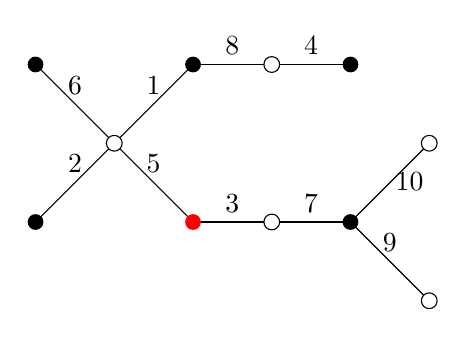
\begin{tikzpicture}
\coordinate (6) at (0,1);
\coordinate (2) at (0,-1);
\coordinate (1) at (2,1);
\coordinate (5) at (1,0);
\coordinate (8) at (3,1);
\coordinate (4) at (4,1);
\coordinate (3) at (3,-1);
\coordinate (7) at (4,-1);
\coordinate (9) at (5,-2);
\coordinate (10) at (5,0);
\coordinate (r) at (2,-1);
\draw (6)--(5) node[midway, above]{6};
\draw (2)--(5) node[midway, above]{2};
\draw (1)--(5) node[midway, above]{1};
\draw (r)--(5) node[midway, above]{5};
\draw (r)--(3) node[midway, above]{3};
\draw (3)--(7) node[midway, above]{7};
\draw (7)--(9) node[midway, above]{9};
\draw (7)--(10) node[near end, below]{10};
\draw (1)--(8) node[midway, above]{8};
\draw (8)--(4) node[midway, above]{4};
\fill (6) circle(0.1);
\fill (2) circle(0.1);
\fill (1) circle(0.1);
\fill[red] (r) circle(0.1);
\fill (4) circle(0.1);
\fill (7) circle(0.1);
\fill[draw,fill=white] (5) circle(0.1);
\fill[draw,fill=white] (3) circle(0.1);
\fill[draw,fill=white] (8) circle(0.1);
\fill[draw,fill=white] (9) circle(0.1);
\fill[draw,fill=white] (10) circle(0.1);
\end{tikzpicture}
\hspace{1cm}
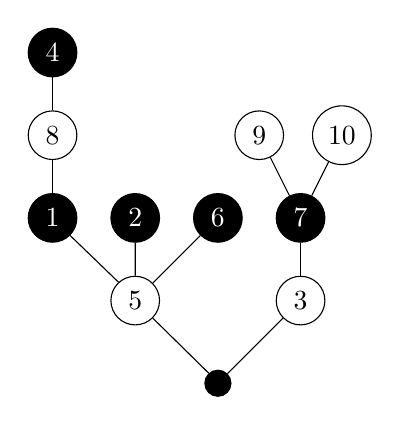
\begin{tikzpicture}[grow=up, scale=0.7,  level 1/.style={sibling distance=3cm},
    level 2/.style={sibling distance=1.5cm}]
\node[draw, circle, fill=black]{}
   child{node[draw, circle]{3}
      child{node[draw, circle, fill=black, text=white]{7}
         child{node[draw, circle]{10}
         }
         child{node[draw, circle]{9}}
      }   
   }
   child{node[draw, circle]{5}
      child{node[draw, circle, fill=black, text=white]{6}
      }   
      child{node[draw, circle, fill=black, text=white]{2}
      }   
      child{node[draw, circle, fill=black, text=white]{1}
         child{node[draw, circle]{8}
            child{node[draw, circle, fill=black, text=white]{4}}         
         }
      }   
   };
\end{tikzpicture}
\end{center}
Separating corollas with a Pr\"ufer algorithm, we get the word $1 \bullet 7 7$ and the following set of corollas:
\begin{equation*}
\left \lbrace 
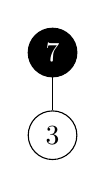
\begin{tikzpicture}[grow=up, scale=0.7, baseline=10]
\node[draw, circle]{3}
      child{node[draw, circle, fill=black, text=white]{7}};
 \end{tikzpicture},
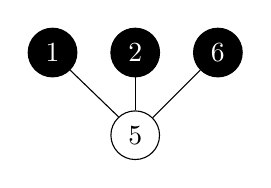
\begin{tikzpicture}[grow=up, scale=0.7, baseline=10]
\node[draw, circle]{5}
      child{node[draw, circle, fill=black, text=white]{6}
      }   
      child{node[draw, circle, fill=black, text=white]{2}
      }   
      child{node[draw, circle, fill=black, text=white]{1}
      }   ;
 \end{tikzpicture}, 
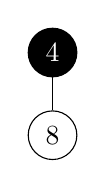
\begin{tikzpicture}[grow=up, scale=0.7, baseline=10]
\node[draw, circle]{8}
            child{node[draw, circle, fill=black, text=white]{4}} ;
 \end{tikzpicture},
 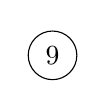
\begin{tikzpicture}[grow=up, scale=0.7, baseline=10]
\node[draw, circle]{9};
 \end{tikzpicture},
  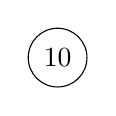
\begin{tikzpicture}[grow=up, scale=0.7, baseline=10]
\node[draw, circle]{10};
 \end{tikzpicture}
  \right \rbrace
\end{equation*}
This set of corollas can be viewed as a function $f$ from the set of labelled black vertices $\{1,2,4,6,7\}$ to the set of white vertices $\{3,5,8,9,10\}$ satisfying $f(1)=f(2)=f(6)=5$, $f(7)=3$ and $f(4)=8$.
\end{example}





\bigskip 

\emph{Acknowledgements.}    

\bibliographystyle{amsalpha}

\bibliography{Poissons}

\end{document}